\begin{center}
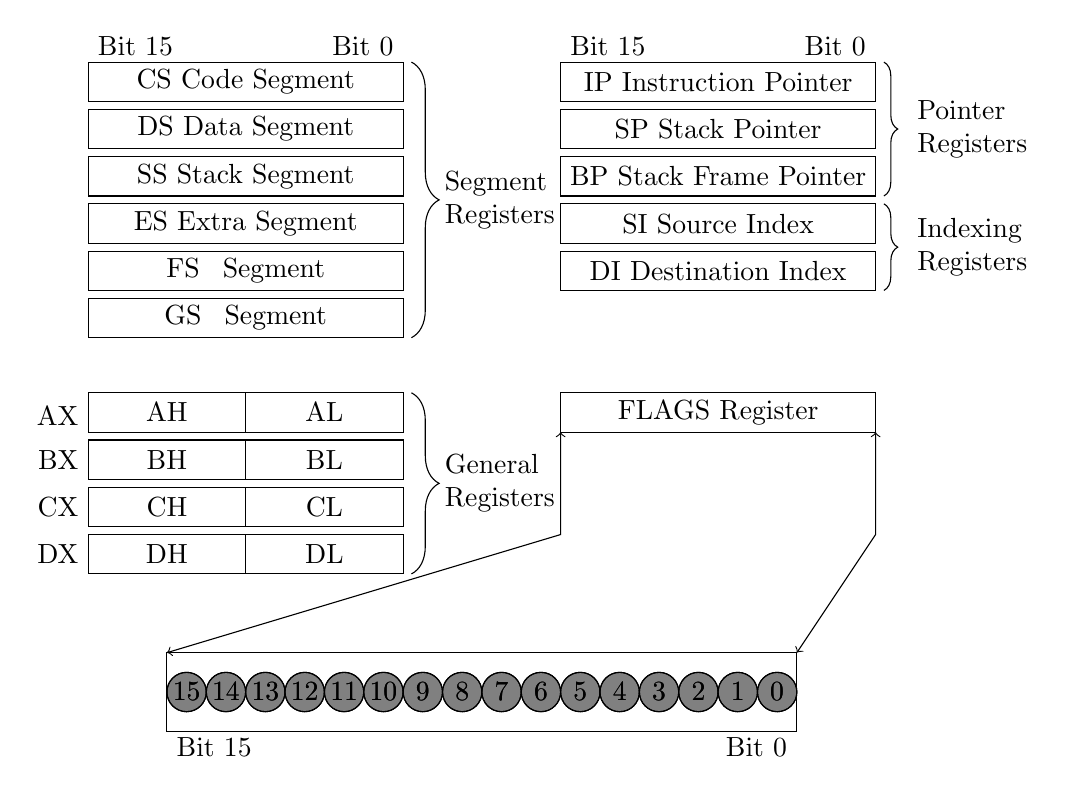
\begin{tikzpicture}
\node[left] at (0,0.25) {DX};
\draw (0,0) rectangle (2,.5) node [pos=0.5] {DH};
\draw (2,0) rectangle (4,.5) node [pos=0.5] {DL};

\node[left] at (0,0.85) {CX};
\draw (0,0.6) rectangle (2,1.1) node [pos=0.5] {CH};
\draw (2,0.6) rectangle (4,1.1) node [pos=0.5] {CL};

\node[left] at (0,1.45) {BX};
\draw (0,1.2) rectangle (2,1.7) node [pos=0.5] {BH};
\draw (2,1.2) rectangle (4,1.7) node [pos=0.5] {BL};

\node[left] at (0,2) {AX};
\draw (0,1.8) rectangle (2,2.3) node [pos=0.5] {AH};
\draw (2,1.8) rectangle (4,2.3) node [pos=0.5] {AL};

\draw [decorate,decoration={brace,amplitude=10pt,mirror},xshift=3pt,yshift=0pt]
(4,0) -- (4,2.3) node [black,midway,right,xshift=0.3cm,text width=1.5cm] 
{General Registers};

\draw (0,3) rectangle (4,3.5) node [pos=0.5] {GS \, Segment};
\draw (0,3.6) rectangle (4,4.1) node [pos=0.5] {FS \, Segment};
\draw (0,4.2) rectangle (4,4.7) node [pos=0.5] {ES Extra Segment};
\draw (0,4.8) rectangle (4,5.3) node [pos=0.5] {SS Stack Segment};
\draw (0,5.4) rectangle (4,5.9) node [pos=0.5] {DS Data Segment};
\draw (0,6) rectangle (4,6.5) node [pos=0.5] {CS Code Segment};

\draw [decorate,decoration={brace,amplitude=10pt,mirror},xshift=3pt,yshift=0pt]
(4,3) -- (4,6.5) node [black,midway,right,xshift=0.3cm,text width=1.5cm] 
{Segment Registers};

\node [right] at (0,6.7) {Bit 15};
\node [left] at (4,6.7) {Bit 0};

\draw (6,1.8) rectangle (10,2.3) node [pos=0.5] {FLAGS Register};

\draw (6,3.6) rectangle (10,4.1) node [pos=0.5] {DI Destination Index};
\draw (6,4.2) rectangle (10,4.7) node [pos=0.5] {SI Source Index};
\draw (6,4.8) rectangle (10,5.3) node [pos=0.5] {BP Stack Frame Pointer};
\draw (6,5.4) rectangle (10,5.9) node [pos=0.5] {SP Stack Pointer};
\draw (6,6) rectangle (10,6.5) node [pos=0.5] {IP Instruction Pointer};
\draw [decorate,decoration={brace,amplitude=5pt,mirror},xshift=3pt,yshift=0pt]
(10,4.8) -- (10,6.5) node [black,midway,right,xshift=0.3cm,text width=1.5cm] 
{Pointer Registers};
\draw [decorate,decoration={brace,amplitude=5pt,mirror},xshift=3pt,yshift=0pt]
(10,3.6) -- (10,4.7) node [black,midway,right,xshift=0.3cm,text width=1.5cm] 
{Indexing Registers};

\node [right] at (6,6.7) {Bit 15};
\node [left] at (10,6.7) {Bit 0};

\draw (1,-1) rectangle (9,-2);
\draw[<->] (6,1.8) -- (6,0.5) -- (1,-1);
\draw[<->] (10,1.8) -- (10,0.5) -- (9,-1);

\foreach \x in {15,...,0}
	\ifthenelse{9 = \x \OR  8 = \x}
	{\draw[fill=gray] (8-\x/2+.75,-1.5) node (B\x) {\x} circle (0.25);}
	{\draw (8-\x/2+.75,-1.5) node (B\x) {\x} circle (0.25);};

	
\node [right] at (1,-2.2) {Bit 15};
\node [left] at (9,-2.2) {Bit 0};
\end{tikzpicture}
\end{center}